\documentclass[12pt]{article}
\usepackage{latexsym,amssymb,amsmath} % for \Box, \mathbb, split, etc.
% \usepackage[]{showkeys} % shows label names
\usepackage{cite} % sorts citation numbers appropriately
\usepackage{path}
\usepackage{url}
\usepackage{verbatim}
\usepackage{float}
\usepackage{subfig}
\usepackage[pdftex]{graphicx}
\usepackage{hyperref}

\usepackage{xcolor}
\hypersetup{
	colorlinks,
	linkcolor={red!50!black},
	citecolor={blue!50!black},
	urlcolor={blue!80!black}
}


% horizontal margins: 1.0 + 6.5 + 1.0 = 8.5
\setlength{\oddsidemargin}{0.0in}
\setlength{\textwidth}{6.5in}
% vertical margins: 1.0 + 9.0 + 1.0 = 11.0
\setlength{\topmargin}{0.0in}
\setlength{\headheight}{12pt}
\setlength{\headsep}{13pt}
\setlength{\textheight}{625pt}
\setlength{\footskip}{24pt}

\renewcommand{\textfraction}{0.10}
\renewcommand{\topfraction}{0.85}
\renewcommand{\bottomfraction}{0.85}
\renewcommand{\floatpagefraction}{0.90}

\makeatletter
\setlength{\arraycolsep}{2\p@} % make spaces around "=" in eqnarray smaller
\makeatother

% change equation, table, figure numbers to be counted inside a section:
\numberwithin{equation}{section}
\numberwithin{table}{section}
\numberwithin{figure}{section}

% begin of personal macros
\newcommand{\half}{{\textstyle \frac{1}{2}}}
\newcommand{\eps}{\varepsilon}
\newcommand{\myth}{\vartheta}
\newcommand{\myphi}{\varphi}

\newcommand{\IN}{\mathbb{N}}
\newcommand{\IZ}{\mathbb{Z}}
\newcommand{\IQ}{\mathbb{Q}}
\newcommand{\IR}{\mathbb{R}}
\newcommand{\IC}{\mathbb{C}}
\newcommand{\Real}[1]{\mathrm{Re}\left({#1}\right)}
\newcommand{\Imag}[1]{\mathrm{Im}\left({#1}\right)}

\newcommand{\norm}[2]{\|{#1}\|_{{}_{#2}}}
\newcommand{\abs}[1]{\left|{#1}\right|}
\newcommand{\ip}[2]{\left\langle {#1}, {#2} \right\rangle}
\newcommand{\der}[2]{\frac{\partial {#1}}{\partial {#2}}}
\newcommand{\dder}[2]{\frac{\partial^2 {#1}}{\partial {#2}^2}}

\newcommand{\nn}{\mathbf{n}}
\newcommand{\xx}{\mathbf{x}}
\newcommand{\uu}{\mathbf{u}}

\newcommand{\junk}[1]{{}}

% set two lengths for the includegraphics commands used to import the plots:
\newlength{\fwtwo} \setlength{\fwtwo}{0.45\textwidth}
% end of personal macros

\begin{document}
\DeclareGraphicsExtensions{.jpg}

\begin{center}
%\textbf{\Large Crop/Weed Classification in (CWFID) Image Dataset using some Machine Learning techniques through image representation in Bag-of-visual-words (BOW), Vector of Locally Aggregated Descriptors (VLAD) and Fisher Vector (FV)\newline\newline(Machine Learning Final Project)} \\[6pt]

\textbf{\Large Comparison of some image representation strategies and Machine Learning algorithms for Crop/Weed classification in the (CWFID) image dataset \newline\newline(Machine Learning Final Project)} \\[6pt]

%\textbf{\Large Crop rows segmentation in sugarcane fields through computer vision techniques \newline \newline  Pattern Recognition Final Project} \\[6pt]
  Fabio Andres Herrera \\[6pt]
  Escuela de Ingeniería de Sistemas y Computación\\
  Universidad del Valle, Cali - Colombia  \\[6pt]
  fabio.herrera@correounivalle.edu.co
  %, \url{www.math.umbc.edu/~gobbert}
\end{center}

\begin{abstract}
\noindent	
This report presents a simple academic exercise were a set of SIFT descriptors was extracted from a group of phenotyping crop/weed image dataset using computer vision techniques. A Bag-of-visual-words model (BovW), Vector of Locally Aggregated Descriptors (VLAD) and a Fisher Vector (FV) encoding are used for image representation. For image classification purposes some machine learning classifiers such as (Gaussian Naive Bayes, Random Forest, Multi-layer Perceptron among others ) were used for crop/weed classification in the CWFID\footnote{Crop/Weed Field Image Dataset for the Evaluation of Computer Vision Based Precision Agriculture Tasks.} image dataset of top-down looking images of organic carrots. A  mean accuracy and a confusion matrix on the given test data and labels are used as an evaluation metric to allow comparison of different algorithms used for classification.

%. The Crop /Weed Field Image Dataset (CWFID) comprises 60 images with annotations with a ground truth vegetation segmentation mask and manual annotation of the plant type (crop vs. weed)

\end{abstract}

\subparagraph{\textit{Key words.}}\textit{Computer Vision, Machine Learning, Phenotyping, Precision Agriculture}

%https://www.cs.princeton.edu/courses/archive/spr08/cos511/scribe_notes/0204.pdf

\section{Introduction}

Machine learning is the science of getting computers to act without being explicitly programmed\cite{5392560}. Machine learning is about learning to do better in the future based on what was experienced in the past. The process of learning begins with observations or data, such as examples, direct experience, or instruction, in order to look for patterns in data and make better decisions in the future based on the examples that we provide. Machine learning is a core subarea of artificial intelligence. Machine learning algorithms are often categorized as supervised or unsupervised \cite{Ratsch2004}.

\begin{itemize}
	\item \textbf{Supervised machine learning :}
	can apply what has been learned in the past to new data using labeled examples to predict future events. Starting from the analysis of a known training dataset, the learning algorithm produces an inferred function to make predictions about the output values. The system is able to provide targets for any new input after sufficient training. The learning algorithm can also compare its output with the correct, intended output and find errors in order to modify the model accordingly.
	
	\item \textbf{Unsupervised machine learning :}
	are used when the information used to train is neither classified nor labeled. Unsupervised learning studies how systems can infer a function to describe a hidden structure from unlabeled data. The system doesn’t figure out the right output, but it explores the data and can draw inferences from datasets to describe hidden structures from unlabeled data.
	
	\item \textbf{Semi-supervised machine learning :}
	fall somewhere in between supervised and unsupervised learning, since they use both labeled and unlabeled data for training – typically a small amount of labeled data and a large amount of unlabeled data. The systems that use this method are able to considerably improve learning accuracy. Usually, semi-supervised learning is chosen when the acquired labeled data requires skilled and relevant resources in order to train it / learn from it. Otherwise, acquiring unlabeled data generally doesn’t require additional resources.
	
	\item \textbf{Reinforcement machine learning :}
	is a learning method that interacts with its environment by producing actions and discovers errors or rewards. Trial and error search and delayed reward are the most relevant characteristics of reinforcement learning. This method allows machines and software agents to automatically determine the ideal behavior within a specific context in order to maximize its performance. Simple reward feedback is required for the agent to learn which action is best; this is known as the reinforcement signal.
	
	
\end{itemize}

\noindent
Machine learning enables analysis of massive quantities of data. The emphasis of machine learning is on automatic methods. In other words, the goal is to devise learning algorithms that do the learning automatically without human intervention or assistance. There are many examples of machine learning problems. Here are several examples:


\begin{itemize}
	\item \textbf{Optical character recognition:} categorize images of handwritten characters 
	\item \textbf{Face detection:} find faces or indicate if a face is present in images 
	\item \textbf{Spam filtering:} identify email messages as spam or non-spam
	\item \textbf{Topic spotting:} categorize news articles
	\item \textbf{Medical diagnosis:} diagnose a patient as a sufferer or non-sufferer of some disease
	\item \textbf{Customer segmentation:} predict which customers will respond to a promotion
	\item \textbf{Fraud detection:} identify credit card transactions which may be fraudulent
	\item \textbf{Weather prediction:} predict, for instance, whether or not it will rain tomorrow
\end{itemize}


The entire process of a typical learning problem is depicted in Figure \ref{figure4}.
\begin{figure}[H] \centering
	\caption{Diagram of a typical learning problem. }
	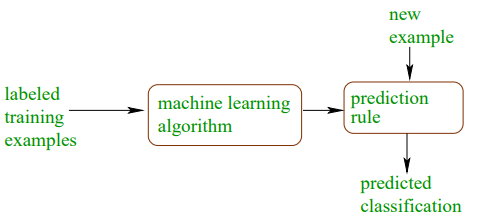
\includegraphics[width=0.6\textwidth]{image4.png}
	\label{figure4}
\end{figure}

\noindent
There are literally thousands of learning algorithms available. The key to not getting lost in this huge space is to realize that it consists of combinations of just three components \cite{Domingos2012}. The components are:

\begin{itemize}

\item \textbf{Representation:} A classifier must be represented in some formal language that the computer can handle. This set is called the hypothesis space of the learner. If a classifier is not in the hypothesis space, it cannot be learned. 

\item \textbf{Evaluation:} An evaluation function (also called scoring function) is needed to distinguish good classifiers from bad ones.The evaluation function used internally by the algorithm may differ from the external one that the classifier want to optimize.

\item \textbf{Optimization:} A method to search among the classifiers in the language for the highest-scoring one. The choice of optimization technique is key to the efficiency of the learner, and also helps determine the classifier produced if the evaluation function has more than one optimum.
\end{itemize}



\section{Scale-invariant feature transform (SIFT) descriptor} \label{sift}
The scale-invariant feature transform (SIFT) is an algorithm in computer vision to detect and describe local features in images. A SIFT descriptor is a 3-D spatial histogram of the image gradients in characterizing the appearance of a keypoint. The gradient at each pixel is regarded as a sample of a three-dimensional elementary feature vector, formed by the pixel location and the gradient orientation. Samples are weighed by the gradient norm and accumulated in a 3-D histogram h, which (up to normalization and clamping) forms the SIFT descriptor of the region. An additional Gaussian weighting function is applied to give less importance to gradients farther away from the keypoint center. Orientations are quantized into eight bins and the spatial coordinates into four each, as seen in Figure \ref{figure6}:

\begin{figure}[H] \centering
	\caption{The SIFT descriptor is a spatial histogram of the image gradient \cite{sift}. }
	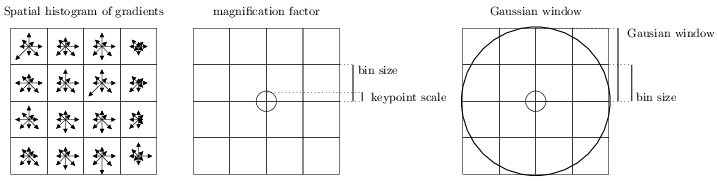
\includegraphics[width=1\textwidth]{image6.png}
	\label{figure6}
\end{figure}

\noindent
The SIFT descriptor is invariant to translations, rotations and scaling transformations in the image domain and robust to moderate perspective transformations and illumination variations.
\noindent
SIFT, as described in \cite{Ke2003}, consists of four major stages:

\begin{itemize}
	\item Scale-space peak selection.
	\item Keypoint localization.
	\item Orientation assignment.
	\item Keypoint descriptor.
\end{itemize}

\noindent
In the first stage, potential interest points are identified by scanning the image over location and scale. This is implemented efficiently by constructing a Gaussian pyramid and searching for local peaks in a series of difference-of-Gaussian (DoG) images. In the second stage, candidate keypoints are localized to sub-pixel accuracy and eliminated if found to be unstable. The third identifies the dominant orientations for each keypoint based on its local image patch. The assigned orientation(s), scale and location for each keypoint enables SIFT to construct a canonical view for the keypoint that is invariant to similarity transforms. The final stage builds a local image descriptor for each keypoint, based upon the image gradients in its local neighborhood. The final (keypoint descriptor) stage of the SIFT algorithm builds a representation for each keypoint based on a patch of pixels in its local neighborhood. Keypoint descriptors typically uses a set of 16 histograms, aligned in a 4x4 grid, each with 8 orientation bins, one for each of the main compass directions and one for each of the mid-points of these directions. This results in a feature vector containing 128 elements. This 128-element vector is then normalized to unit length and thresholded to remove elements with small values.  it is fairly compact, expressing the patch of pixels using a 128 element vector as seen in Figure \ref{sit1}.

\begin{itemize}
	\item {{There is an example of extraction of SIFT descriptors for a single image of the crop/weed dataset:} } \url{https://github.com/AndresHerrera/Proyecto_MachineLearning/blob/master/JupyterNotebook/SIFT_Descriptors.ipynbb}
\end{itemize}

\begin{figure}[H] \centering
	\caption{A single image of the dataset includes crop, weed, and background (soil). }
	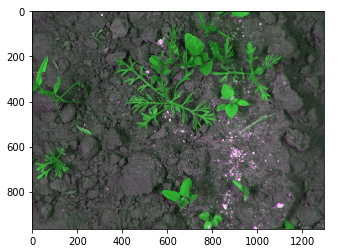
\includegraphics[width=0.5\textwidth]{plant.png}
	\label{plant}
\end{figure}

\noindent
For extraction descriptors, an image annotation mask was used (Figure \ref{mask}). Soil background was removed using image preprocessing.

\begin{figure}[H] \centering
	\caption{Crop/weed mask image annotation - (blue) corresponds to crop and (green) to weed. }
	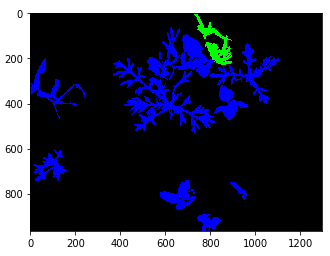
\includegraphics[width=0.5\textwidth]{mask.png}
	\label{mask}
\end{figure}


\begin{figure}[H] \centering
	\caption{A total of 128 bin values represented as a vector to form keypoint descriptor. }
	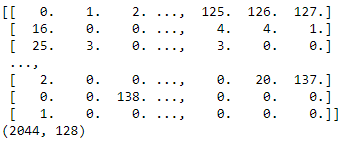
\includegraphics[width=0.5\textwidth]{sift1.png}
	\label{sit1}
\end{figure}







\section{Image vector representation}

Recent works \cite{Arandjelovic2013}, \cite{Delhumeau2013}, \cite{Sanchez2013}, \cite{Singh2012}, \cite{Ke2003} on image retrieval and classification have proposed to index images by compact representations encoding powerful local descriptors, such as the closely related VLAD,  Fisher vector, and Bag of visual words. By combining such a representation with a suitable coding technique, it is possible to encode an image in a few dozen bytes while achieving excellent retrieval or classification results. 

\subsection{Bag of Visual Words (BovW)} \label{bow}

To represent an image using the BovW model (Figure \ref{boww}), an image can be treated as a document. Similarly, "words" in images need to be defined too. To achieve this, it usually includes following three steps: \textbf{feature detection}, \textbf{feature description}, and \textbf{codebook generation}. A definition of the BoW model can be the "histogram representation based on independent features".

\begin{figure}[H] \centering
	\caption{The bag-of-visual-words technique. Image source \cite{mathw}. }
	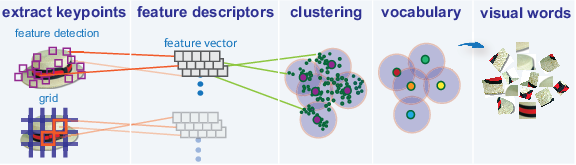
\includegraphics[width=1\textwidth]{bagoffeatures_visualwordsoverview.png}
	\label{boww}
\end{figure}


\begin{itemize}

\item \textbf{Feature representation} After feature detection, each image is abstracted by several local patches. Feature representation methods deal with how to represent the patches as numerical vectors. These vectors are called feature descriptors. A good descriptor should have the ability to handle intensity, rotation, scale and affine variations to some extent. One of the most famous descriptors is Scale-invariant feature transform (SIFT). SIFT converts each patch to 128-dimensional vector. After this step, each image is a collection of vectors of the same dimension (128 for SIFT), where the order of different vectors is of no importance.

\item \textbf{Codebook generation} The final step for the BovW model is to convert vector-represented patches to "codewords" (analogous to words in text documents), which also produces a "codebook" (analogy to a word dictionary). A codeword can be considered as a representative of several similar patches. One simple method is performing k-means clustering over all the vectors. Codewords are then defined as the centers of the learned clusters. The number of the clusters is the codebook size (analogous to the size of the word dictionary).

\end{itemize}

\noindent
Thus, each patch in an image is mapped to a certain codeword through the clustering process and the image can be represented by the histogram of the codewords.





\subsection{Vector of Locally Aggregated Descriptors (VLAD) } \label{vlad}

VLAD is constructed as follows: regions are extracted from an image using an affine invariant detector, and described using the 128-D SIFT descriptor. Each descriptor is then assigned to the closest cluster of a vocabulary of size $k$ (where $k$ is typically 64 or 256, so that clusters are quite coarse). For each of the k clusters, the residuals (vector differences between descriptors and cluster centers) are accumulated, and the $k$ 128-D sums of residuals are concatenated into a single $k$ × 128 dimensional descriptor \cite{Arandjelovic2013}.The vector of locally aggregated descriptors (VLAD) is an encoding technique that produces a fixed-length vector representation $v$ from a set $X = {x1, . . . , xn}$ of n local d-dimensional descriptors, e.g., SIFTs, extracted from a given image \cite{Delhumeau2013}.Vector of locally aggregated descriptors(VLAD), which indexes images to compact representations by aggregating the residuals of descriptors. In the construction of VLAD, each descriptor is first assigned to the closest visual word in a visual codebook in the same way as in the construction of the BovW vector\cite{Uchida2013}.
Initially, VLAD takes all feature descriptors from all training images as inputs to cluster them and find a fixed number of centroids by K-means. The collection of these centroids is referred to as the codebook. To encode an image using the codebook, the details of processing are elaborated as follows. Let $N$ denote the total number of centroids, and $ci(i=1…N)$ denote the centroids. For further information about VLAD \cite{Arandjelovic2013}, \cite{Jegou2010} and \cite{Singh2012} are useful. VLAD adopts SIFT as the feature descriptors for encoding. SIFT is a well-known feature descriptor which is widely applied in computer vision, object recognition and machine intelligence due to its feature distinctness, robustness, and scale and rotation invariant\cite{Singh2012}.

% Similar as BovW model, VLAD aims at representing one single image by a fixed number of feature vectors aggregated by all feature descriptors extracted from this image. Such a representation is called a VLAD encoding for an image. 


\subsection{Fisher Vector (FV)} \label{fv}

Fisher vector encoding is based on a visual dictionary learning method using Gaussian Mixture Models (GMM) \cite{Diba}.
The basic idea of Fisher vector codding (FVC) is to first construct a generative model of local features and use the gradient of the log-likelihood of a particular feature with respect to the model parameters as the feature’s coding vector. When applied as an image representation the FVC vectors of local features are calculated by a pooling operation and normalization to generate the final image representation. FVC has been established as one of the most powerful local feature encoding and image representation generation methods. Gaussian mixture model (GMM) is adopted as the generative model for modeling the local features. The GMM essentially assumes that each local feature is generated from one of the Gaussian distributions in the GMM, and intuitively the mean of each Gaussian distribution serves as a prototype for the local features. Since the dimensionality of the image representation resulting from GMM based FVC is the product of the local feature dimensionality and the number of Gaussians, to make the image representation dimensionality tractable, the number of Gaussians is usually chosen to be few hundred \cite{Liu2016}.\\\\

%http://what-when-how.com/computer-visionimaging-and-computer-graphics/fisher-vectors-beyond-bag-of-visual-words-image-representations-computer-visionimaging-and-computer-graphics-part-1/

%https://www.quora.com/What-is-a-Fisher-vector

%They model the visual words with a Gaussian mixture model (GMM), restricted to diagonal variance matrices for each of the k components of the mixture. Deriving a diagonal approximation of the Fisher matrix of a GMM, they obtain a (2d + 1) × k − 1 dimensional vector representation of an image feature set, or d×kdimensional when considering only the components associated with either the means or the variances of the GMM
\noindent
The Fisher Vector (FV) can be used to describe an entire image for image classification \cite{Sanchez2013}. \\\\

\begin{figure}[H] \centering
	\caption{ Fisher vector encoding. }
	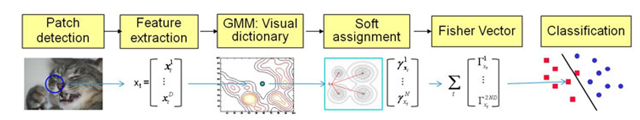
\includegraphics[width=1\textwidth]{fisher.png}
	\label{fisher}
\end{figure}


\begin{itemize}
	\item A Gaussian Mixture Model (GMM) is used to model the distribution of features (e.g. SIFT) extracted all over the image.
	\item The Fisher Vector (FV) encodes the gradients of the log-likelihood of the features under the GMM, with respect to the GMM parameters.
\end{itemize}

\noindent
Since the GMM parameters represent the first-order moments of the features, the FV encodes second-order moments of the features, roughly. Fisher Vector with GMM can be seen as an extension of BovW. Actually, it accumulates the relative position to each cluster center, and models codeword assignment uncertainty, which has shown to be beneficial for BovW encoding\cite{Sun2013}.


%representation of images based on an intermediate representation, the visual vocabulary built in the low level feature space.







\section{Classification Algorithms} \label{classalgs}

\subsection{k-Nearest Neighbor (k-NN)} \label{knn}
The simplest method is the k-Nearest Neighbor classifier. Here the k points of the training data closest to the test point are found, and a label is given to the test point by a majority vote between the k points. This method is highly intuitive and attains – given its simplicity – remarkably low classification errors, but it is computationally expensive and requires a large memory to store the training data. k-NN makes predictions using the training dataset directly. Predictions are made for a new instance $(x)$ by searching through the entire training set for the $K$ most similar instances (the neighbors) and summarizing the output variable for those $k$ instances. For regression this might be the mean output variable, in classification this might be the mode (or most common) class value. To determine which of the $k$ instances in the training dataset are most similar to a new input a distance measure is used. For real-valued input variables, the most popular distance measure is \textbf{Euclidean distance}. Euclidean distance is calculated as the square root of the sum of the squared differences between a new point $(x)$ and an existing point $(xi)$ across all input attributes $j$.
$EuclideanDistance(x, xi) = sqrt( sum( (xj – xij)^2 ) )$

\begin{figure}[H] \centering
	\caption{ Efficiency of the k-NN algorithm largely depends on the value of k nearest neighbors. }
	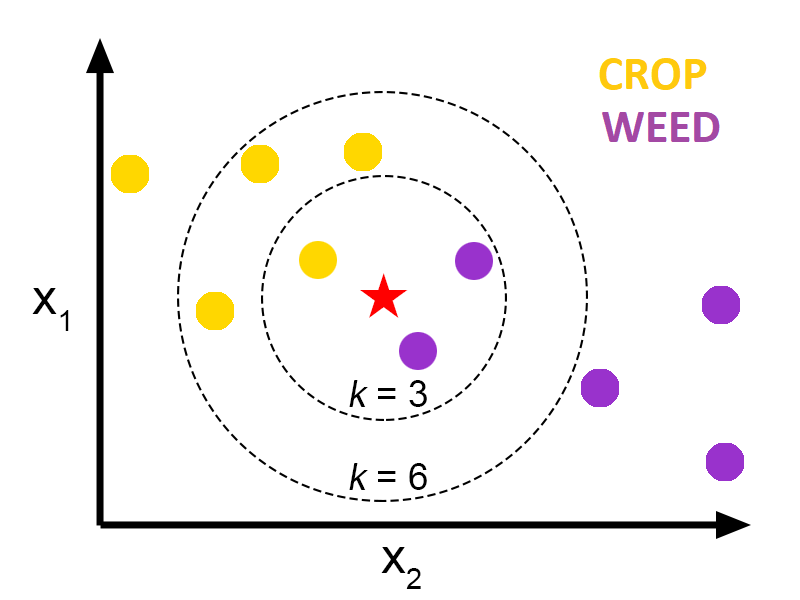
\includegraphics[width=0.4\textwidth]{r_knn_concept.png}
	\label{knnn}
\end{figure}

\noindent
Other popular distance measures include:

\begin{itemize}
	\item Hamming Distance: Calculate the distance between binary vectors.
	\item Manhattan Distance: Calculate the distance between real vectors using the sum of their absolute difference.
	\item Minkowski Distance: Generalization of Euclidean and Manhattan distance.
\end{itemize}




%\subsection{Linear Discriminant Analysis} \label{lda}
%computes a hyperplane in the input space that minimizes the within-class variance and maximizes the between class distance. It can be efficiently computed in the linear case even with large data sets. However, often a linear separation is not sufficient. Nonlinear extensions by using kernels exist, however, making it difficult to apply it to problems with large training sets.

%\subsection{Decision Trees} \label{dectree}
%These algorithms solve the classification problem by repeatedly partitioning the in put space, so as to build a tree whose nodes are as pure as possible (that is, they contain points of a single class). Classification of a
%new test point is achieved by moving from top to bottom along the branches of the tree, starting from the root node, until a terminal node is reached. Decision trees are simple yet effective classification schemes for small datasets. The computational complexity scales unfavorably with the number of dimensions of the data. Large datasets tend to result in complicated trees, which in turn require a large memory for storage. 

\subsection{Random Forest} \label{randomf}

Random forests is an ensemble model which means that it uses the results from many different models to calculate a response. In most cases the result from an ensemble model will be better than the result from any one of the individual models. In the case of random forests, several decision trees are created (grown) and the response is calculated based on the outcome of all of the decision trees \cite{Horning2010}.   A random forest multi-way classifier consists of a number of trees, with each tree grown using some form of randomization. The leaf nodes of each tree are labeled by estimates of the posterior distribution over the image classes. Each internal node contains a test that best splits the space of data to be classified. An image is classified by sending it down every tree and aggregating the reached leaf distributions. Randomness can be injected at two points during training: in subsampling the training data so that each tree is grown using a different subset; and in selecting the node tests\cite{Bosch2007}.A random forest is a meta estimator that fits a number of decision tree classifiers on various sub-samples of the dataset and use averaging to improve the predictive accuracy and control over-fitting. In order to prevent over-fitting the maximum depth of the tree selected was 2 as seen in the following Jupyter Notebook file:

\begin{itemize}
	\item {\textbf{Random Forest over-fitting :} } \url{https://github.com/AndresHerrera/Proyecto_MachineLearning/blob/master/JupyterNotebook/BagOfVisualWords_RF_Eval.ipynb}
\end{itemize}

\subsubsection{Decision Trees} \label{dectree}
These algorithms solve the classification problem by repeatedly partitioning the in put space, so as to build a tree whose nodes are as pure as possible (that is, they contain points of a single class). Classification of a
new test point is achieved by moving from top to bottom along the branches of the tree, starting from the root node, until a terminal node is reached. Decision trees are simple yet effective classification schemes for small datasets. The computational complexity scales unfavorably with the number of dimensions of the data. Large datasets tend to result in complicated trees, which in turn require a large memory for storage. 



\subsection{Naive Bayes} \label{naive}
%https://www.analyticsvidhya.com/blog/2017/09/naive-bayes-explained/
%http://dataaspirant.com/2017/02/06/naive-bayes-classifier-machine-learning/

It is a classification technique based on Bayes theorem \cite{Triola} with an assumption of independence among predictors. In simple terms, a Naive Bayes classifier assumes that the presence of a particular feature in a class is unrelated to the presence of any other feature. Naive Bayes model is easy to build and particularly useful for very large data sets. Along with simplicity, Naive Bayes is known to outperform even highly sophisticated classification methods. Bayes theorem provides a way of calculating posterior probability $P(c|x)$ from $P(c)$, $P(x)$ and $P(x|c)$. It predicts membership probabilities for each class such as the probability that given record or data point belongs to a particular class.  The class with the highest probability is considered as the most likely class. Naive Bayes classifier assumes that all the features are unrelated to each other. Presence or absence of a feature does not influence the presence or absence of any other feature. For further information about Naive Bayes this survey \cite{Jiang2007} is useful.

\subsection{Neural Networks} \label{neuralnetwork}

Neural networks are a computational model inspired by the connectivity of neurons in animate nervous systems.
A further boost to their popularity came with the proof that they can approximate any function mapping via the Universal Approximation Theorem \cite{Ratsch2004}. 


\subsubsection{The Perceptron} \label{perc}

A perceptron has one or more inputs, a bias, an activation function, and a single output. The perceptron receives inputs, multiplies them by some weight, and then passes them into an activation function to produce an output. There are many possible activation functions to choose from, such as the logistic function, a trigonometric function, a step function among others.

\begin{figure}[H] \centering
	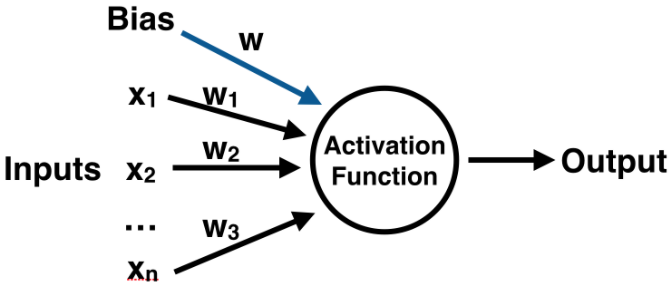
\includegraphics[width=0.4\textwidth]{perceptron.png}
	\caption{A schematic diagram of a neural network. Each circle in the hidden and output layer is a computational element known as a neuron. }
	\label{perceptron}
\end{figure}

\noindent
To create a neural network, layers of perceptrons must be added together, creating a multi-layer perceptron model of a neural network. An input layer which directly takes in your data and an output layer which will create the resulting outputs. Any layers in between are known as hidden layers because they don’t directly “see” the feature inputs within the data you feed in or the outputs.  Multi Layer perceptron (MLP) is a feedforward neural network with one or more layers between input and output layer. Feedforward means that data flows in one direction from input to output layer (forward). This type of network is trained with the backpropagation learning algorithm. MLPs are widely used for pattern classification, recognition, prediction and approximation. Multi Layer Perceptron can solve problems which are not linearly separable. A simple scheme for a MLP neural network is shown in Figure \ref{figure5}. Each circle denotes a computational element referred to as a neuron, which computes a weighted sum of its inputs, and possibly performs a nonlinear function on this sum. If certain classes of nonlinear functions are used, the function computed by the network can approximate any function (specifically a mapping from the training patterns to the training targets), provided enough neurons exist in the network and enough training examples are provided.

\begin{figure}[H] \centering
	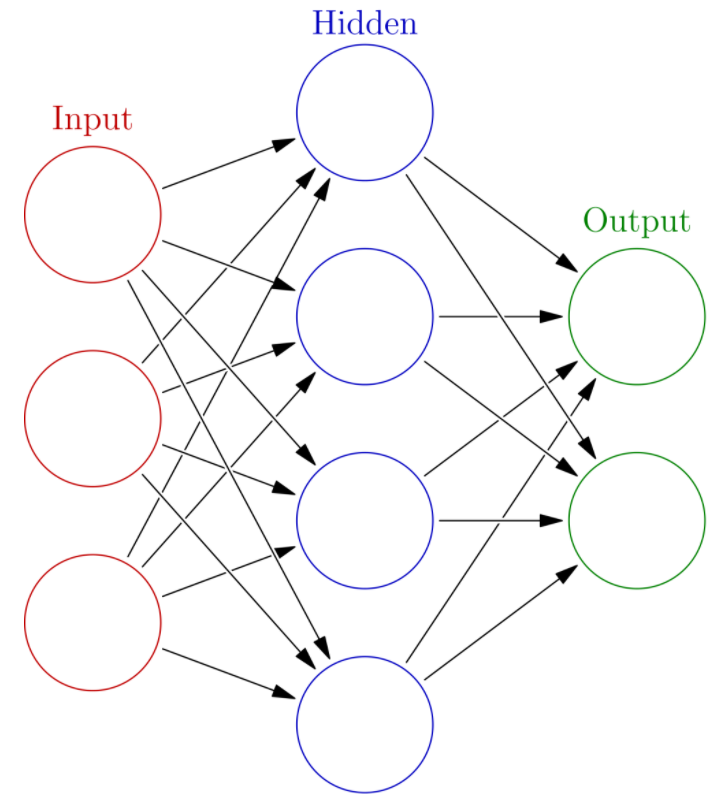
\includegraphics[width=0.3\textwidth]{mlp.png}
	\caption{A schematic diagram of a neural network. Each circle in the hidden and output layer is a computational element known as a neuron. }
	\label{figure5}
\end{figure}





%
%\subsection{Multi-layer Perceptron (MLP)} \label{mlp}
%%https://www.hiit.fi/u/ahonkela/dippa/node41.html
%%http://scikit-learn.org/stable/modules/neural_networks_supervised.html
%
%\begin{figure}[H] \centering
%	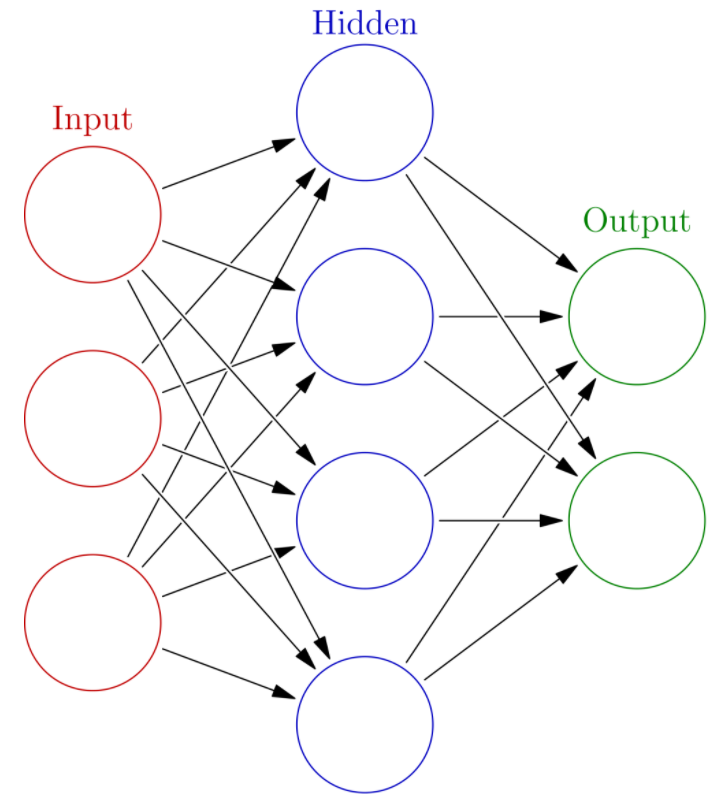
\includegraphics[width=0.4\textwidth]{mlp.png}
%	\caption{Graph of an MLP }
%	\label{mlpg}
%\end{figure}




%\subsection{One-vs-the-rest (OvR) } \label{ovr}
%
%Also known as one-vs-all, this strategy consists in fitting one classifier per class. For each classifier, the class is fitted against all the other classes. In addition to its computational efficiency (only nclasses classifiers are needed), one advantage of this approach is its interpretability. Since each class is represented by one and one classifier only, it is possible to gain knowledge about the class by inspecting its corresponding classifier. This is the most commonly used strategy for multiclass classification and is a fair default choice.
%
%This strategy can also be used for multilabel learning, where a classifier is used to predict multiple labels for instance, by fitting on a 2-d matrix in which cell [i, j] is 1 if sample i has label j and 0 otherwise.
%
%In the multilabel learning literature, OvR is also known as the binary relevance method.

%http://scikit-learn.org/stable/modules/generated/sklearn.multiclass.OneVsRestClassifier.html


\section{Crop and Weed Image Dataset}

The dataset \cite{haug15} comprises field images in top-down view that were acquired with the autonomous field robot Bonirob\cite{BOSH} in an organic carrot farm in 2013. The images were captured while the crop was in growth stages where one or more true leaves were present. All images are annotated and a ground truth vegetation segmentation mask is available together with crop/weed annotations. Figure \ref{figure1} shows a field image (a), a segmentation mask (b) and Crop/weed annotation image (c) even a file in YAML format with a list of polygon vertices and labels.

\begin{figure}[H] \centering
	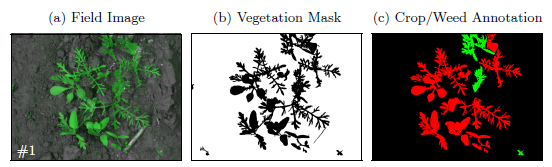
\includegraphics[width=1\textwidth]{image1.png}
	\caption{Sample images from the dataset (a) with ground truth vegetation masks
		and crop /weed annotations. The annotation images (b) and (c) are supplied for
		every image of the dataset. Modified from \cite{Haug2015}. }
	\label{figure1}
\end{figure}


\noindent
The dataset images ware acquired by a JAI multi-spectral camera that captures both visible and near-infrared light was used and mounted on the robot. The camera was looking downwards and the area under the robot was shaded and artificially lit to avoid changing lighting conditions. Figure \ref{figure2} describes the camera setup and its configuration.

\begin{figure}[H] \centering
	\caption{Description of camera system and acquisition parameters. Modified from \cite{Haug2015}. }
	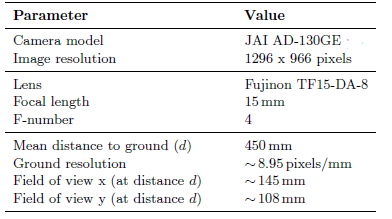
\includegraphics[width=0.6\textwidth]{image2.png}
	\label{figure2}
\end{figure}

\noindent
The Crop /Weed Field Image Dataset (CWFID) was downloaded from:
\begin{itemize}
	\item {\textbf{CWFID Image Dataset:} } \url{http://github.com/cwfid}
	
\end{itemize}

\noindent
The following Jupyter Notebook file shows how the files were read 

\begin{itemize}
	\item {\textbf{Reading Crop and Weed Dataset:} } \url{https://github.com/AndresHerrera/Proyecto_MachineLearning/blob/master/JupyterNotebook/ReadCropWeedDataset.ipynb}
\end{itemize}


\section{Comparison} \label{Comparison}


\begin{figure}[H] \centering
	\caption*{Table 6.1:  Comparison of machine learning classifiers over different image descriptors. }
	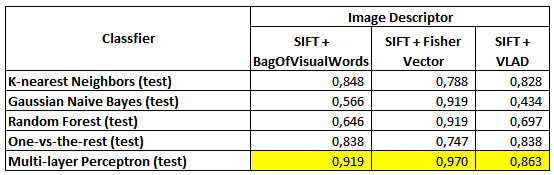
\includegraphics[width=0.8\textwidth]{class.png}
	\label{class}
\end{figure}

\noindent
In multilabel classification, mean accuracy on the given test data and labels.  If the entire set of predicted labels for a sample strictly match with the true set of labels, then the subset accuracy is 1.0; otherwise it is 0.0.

\begin{figure}[H] \centering
	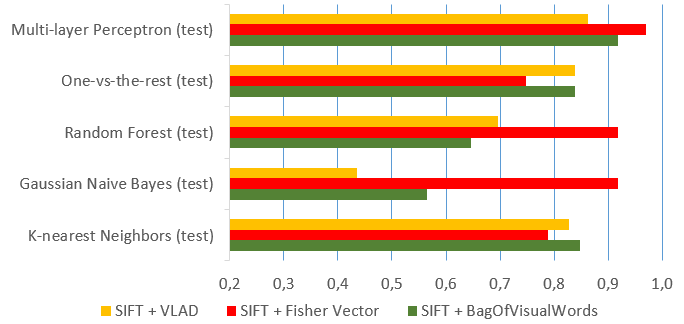
\includegraphics[width=0.8\textwidth]{graph.png}
	\caption{Comparision results of classifiers and Image descriptors (mean accuracy )  }
	\label{graph}
\end{figure}

\section{Confusion Matrix} \label{cmatrix}

A confusion matrix is a table that is often used to describe the performance of a classification model (or "classifier") on a set of test data for which the true values are known.  A classification system has been trained to distinguish between crop and weed(no-crop), a confusion matrix will summarize the results of testing the algorithm for further inspection the resulting confusion matrix could look like the Figure \ref{mtx} below :

\begin{figure}[H] \centering
	\caption{Confusion matrix }
	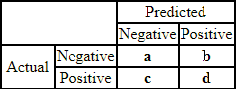
\includegraphics[width=0.33\textwidth]{mtx.png}
	\label{mtx}
\end{figure}

The entries in the confusion matrix have the following meaning in the context of our study:

\begin{itemize}
	\item \textbf{a} is the number of correct predictions that an instance is negative.
	\item \textbf{b} is the number of incorrect predictions that an instance is positive.
	\item \textbf{c} is the number of incorrect of predictions that an instance negative.
	\item \textbf{d} is the number of correct predictions that an instance is positive.
\end{itemize}

\noindent
\textbf{Accuracy : }it is the fraction of correctly classified pixels with regard to all pixels of that ground truth class. For each class of ground truth pixels (row), the number of correctly classified pixels is divided by the total number of ground truth or test pixels of that class. 


\subsection{BagOfVisualWords}

\begin{figure}[H] \centering
	\caption*{Table 7.1: Confusion matrix for K-nearest neighbors classifier. }
	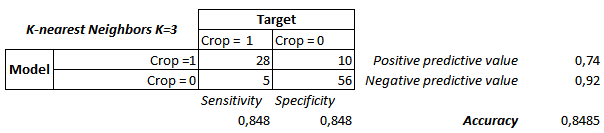
\includegraphics[width=0.8\textwidth]{m1.png}
	\label{m1}
\end{figure}

\begin{figure}[H] \centering
	\caption*{Table 7.2: Confusion matrix for Multi-layer Perceptron classifier. }
	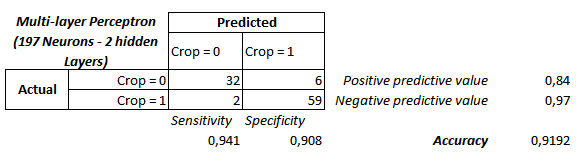
\includegraphics[width=0.8\textwidth]{m2.png}
	\label{m2}
\end{figure}

\begin{figure}[H] \centering
	\caption*{Table 7.3: Confusion matrix for Gaussian Naive Bayes classifier. }
	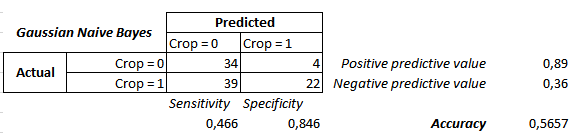
\includegraphics[width=0.8\textwidth]{m3.png}
	\label{m3}
\end{figure}

\begin{figure}[H] \centering
	\caption*{Table 7.4: Confusion matrix for One-vs-the-rest classifier. }
	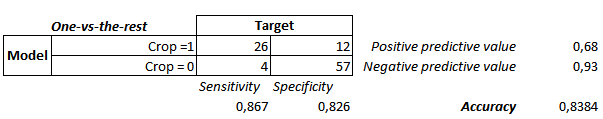
\includegraphics[width=0.8\textwidth]{m4.png}
	\label{m4}
\end{figure}

\begin{figure}[H] \centering
	\caption*{Table 7.5: Confusion matrix for Random Forest classifier. }
	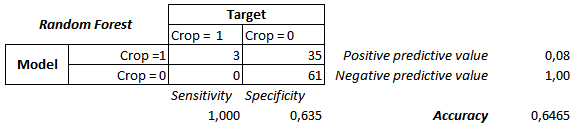
\includegraphics[width=0.8\textwidth]{m5.png}
	\label{m5}
\end{figure}

\subsection{Fisher Vector}

\begin{figure}[H] \centering
	\caption*{Table 7.6: Confusion matrix for K-nearest neighbors classifier. }
	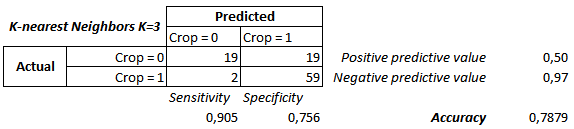
\includegraphics[width=0.8\textwidth]{m6.png}
	\label{m6}
\end{figure}

\begin{figure}[H] \centering
	\caption*{Table 7.7: Confusion matrix for Multi-layer Perceptron classifier. }
	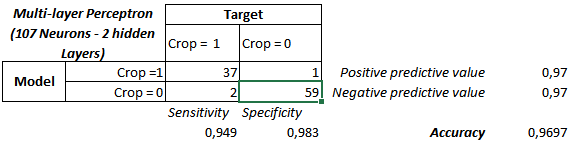
\includegraphics[width=0.8\textwidth]{m7.png}
	\label{m7}
\end{figure}

\begin{figure}[H] \centering
	\caption*{Table 7.8: Confusion matrix for Gaussian Naive Bayes classifier. }
	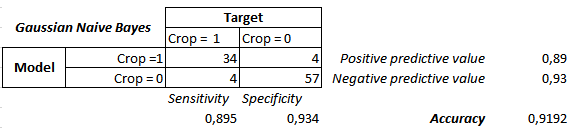
\includegraphics[width=0.8\textwidth]{m8.png}
	\label{m8}
\end{figure}

\begin{figure}[H] \centering
	\caption*{Table 7.9: Confusion matrix for One-vs-the-rest classifier. }
	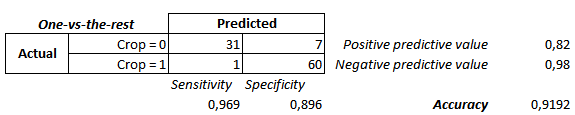
\includegraphics[width=0.8\textwidth]{m9.png}
	\label{m9}
\end{figure}

\begin{figure}[H] \centering
	\caption*{Table 7.10: Confusion matrix for Random Forest classifier. }
	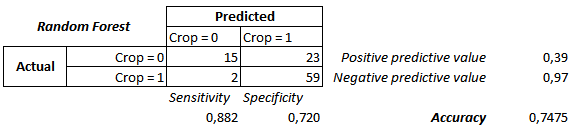
\includegraphics[width=0.8\textwidth]{m10.png}
	\label{m10}
\end{figure}


\subsection{VLAD}

\begin{figure}[H] \centering
	\caption*{Table 7.11: Confusion matrix for K-nearest neighbors classifier. }
	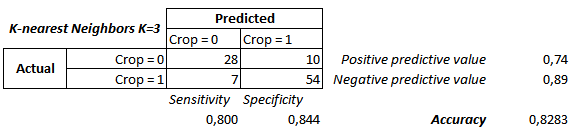
\includegraphics[width=0.8\textwidth]{m11.png}
	\label{m11}
\end{figure}

\begin{figure}[H] \centering
	\caption*{Table 7.12: Confusion matrix for Multi-layer Perceptron classifier. }
	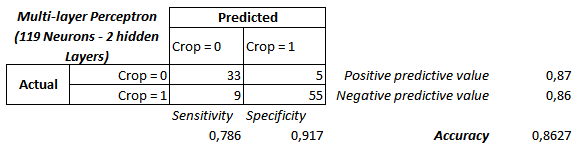
\includegraphics[width=0.8\textwidth]{m12.png}
	\label{m12}
\end{figure}

\begin{figure}[H] \centering
	\caption*{Table 7.13: Confusion matrix for Gaussian Naive Bayes classifier. }
	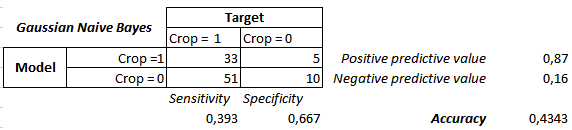
\includegraphics[width=0.8\textwidth]{m13.png}
	\label{m13}
\end{figure}

\begin{figure}[H] \centering
	\caption*{Table 7.14: Confusion matrix for One-vs-the-rest classifier. }
	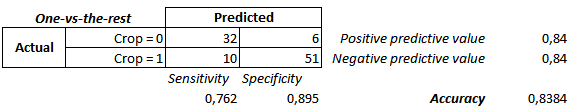
\includegraphics[width=0.8\textwidth]{m14.png}
	\label{m14}
\end{figure}

\begin{figure}[H] \centering
	\caption*{Table 7.15: Confusion matrix for Random Forest classifier. }
	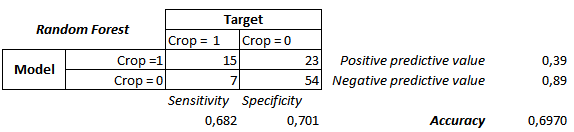
\includegraphics[width=0.8\textwidth]{m15.png}
	\label{m15}
\end{figure}




\section{Source Code Repository}

Python code blocks and running results are available on GitHub over Jupyter Notebooks

\subsection{K-nearest Neighbors Classifier }

\begin{itemize}
	\item {\textbf{BagOfVisualWords - KN :} } \url{https://github.com/AndresHerrera/Proyecto_MachineLearning/blob/master/JupyterNotebook/BagOfVisualWords_KN.ipynb}
	
	\item {\textbf{Fisher Vector - KN :} } \url{	https://github.com/AndresHerrera/Proyecto_MachineLearning/blob/master/JupyterNotebook/FisherVector_KN.ipynb}
	
	\item {\textbf{VLAD - KN :} } \url{	https://github.com/AndresHerrera/Proyecto_MachineLearning/blob/master/JupyterNotebook/VLAD_KN.ipynb}
		
\end{itemize}

\subsection{Gaussian Naive Bayes Classifier }

\begin{itemize}
	\item {\textbf{BagOfVisualWords - NB :} } \url{https://github.com/AndresHerrera/Proyecto_MachineLearning/blob/master/JupyterNotebook/BagOfVisualWords_NB.ipynb}
	
	\item {\textbf{Fisher Vector - NB :} } \url{	https://github.com/AndresHerrera/Proyecto_MachineLearning/blob/master/JupyterNotebook/FisherVector_NB.ipynb}
	
	\item {\textbf{VLAD - NB :} } \url{	https://github.com/AndresHerrera/Proyecto_MachineLearning/blob/master/JupyterNotebook/VLAD_NB.ipynb}
	
\end{itemize}

\subsection{Random Forest Classifier }

\begin{itemize}
	\item {\textbf{BagOfVisualWords - RF :} } \url{https://github.com/AndresHerrera/Proyecto_MachineLearning/blob/master/JupyterNotebook/BagOfVisualWords_RF.ipynb}
	
	\item {\textbf{Fisher Vector - RF :} } \url{	https://github.com/AndresHerrera/Proyecto_MachineLearning/blob/master/JupyterNotebook/FisherVector_RF.ipynb}
	
	\item {\textbf{VLAD - RF :} } \url{	https://github.com/AndresHerrera/Proyecto_MachineLearning/blob/master/JupyterNotebook/VLAD_RF.ipynb}
	
\end{itemize}


\subsection{One-vs-the-rest Classifier }

\begin{itemize}
	\item {\textbf{BagOfVisualWords - OVR :} } \url{https://github.com/AndresHerrera/Proyecto_MachineLearning/blob/master/JupyterNotebook/BagOfVisualWords_OVR.ipynb}
	
	\item {\textbf{Fisher Vector - OVR :} } \url{	https://github.com/AndresHerrera/Proyecto_MachineLearning/blob/master/JupyterNotebook/FisherVector_OVR.ipynb}
	
	\item {\textbf{VLAD - OVR :} } \url{	https://github.com/AndresHerrera/Proyecto_MachineLearning/blob/master/JupyterNotebook/VLAD_OVR.ipynb}
	
\end{itemize}


\subsection{Multi-layer Perceptron Classifier }

\begin{itemize}
	\item {\textbf{BagOfVisualWords - MLP :} } \url{https://github.com/AndresHerrera/Proyecto_MachineLearning/blob/master/JupyterNotebook/BagOfVisualWords_MLP.ipynb}
	
	\item {\textbf{Fisher Vector - MLP :} } \url{	https://github.com/AndresHerrera/Proyecto_MachineLearning/blob/master/JupyterNotebook/FisherVector_MLP.ipynb}
	
	\item {\textbf{VLAD - MLP :} } \url{	https://github.com/AndresHerrera/Proyecto_MachineLearning/blob/master/JupyterNotebook/VLAD_MLP.ipynb}
	
\end{itemize}






\subsection{Jupyter Notebooks}
\begin{itemize}
	\item {\textbf{All Jupyter NoteBook files on GitHub:} } \url{https://github.com/AndresHerrera/Proyecto_MachineLearning/tree/master/JupyterNotebook} 
\end{itemize}

	
	
\section{Conclusions and discussion}

The artificial neural network Multi-layer perceptron performed best results in the crop/weed classification with an accuracy score upper 91\% on the test set in image representation with SIFT + BagOfVisualWords and SIFT + Fisher Vector, likewise, in SIFT + VLAD  was the best one with accuracy score upper 86\%. Gaussian Naive Bayes classifier was the worst performer in SIFT+BagOfVisualWords and SIFT+VLAD image representation, however, in SIFT+Fisher Vector the scoring accuracy was upper 91\%.\\\\
\noindent
The confusion matrix used gave a better idea of what classification model is getting right and was used for summarizing the performance of classification algorithms evaluated. \\\\
\noindent
A combination of Multi-layer Perceptron with SIFT + Fisher Vector gets a richer feature vector from images compared to SIFT + BagOfVisualWords  or  SIFT + VLAD achieving thus an accuracy score upper 97\% on the test set.\\\\
\noindent
The use of BovW, VLAD and FV encodings is justified by the need for increasing efficiency and reducing
computing resources for image matching or classification on a large datasets.

\section*{Acknowledgments}

To Maria Trujillo Ph.D., a teacher in the course Fundamentals of Multimedia Machine Learning for its valuable training along the fall term 2017.
 

\bibliographystyle{siam}
\bibliography{template}

\end{document}

